\subsection{L(X) 的包络代数}

定理 1. 设 \(\alpha: \mathrm{L}(\mathrm{X}) \to \mathrm{A}(\mathrm{X})\) 是扩张 \(\mathbf{X}\) 到 \(\mathrm{A}(\mathrm{X})\) 中的典范单射的唯一李代数同态 (§ 2， no. 2， 命题 1)。设 \(\sigma \colon \mathrm{L}(\mathrm{X}) \to \mathrm{U}(\mathrm{L}(\mathrm{X}))\) 是 \(\mathrm{L}(\mathrm{X})\) 到它的包络代数中的典范映射，并设 \(\beta \colon \mathrm{U}(\mathrm{L}(\mathrm{X})) \to \mathrm{A}(\mathrm{X})\) 是使得 \(\beta \circ \sigma = \alpha\) 的唯一的幺代数同态 (第 I 章， § 2， no. 1， 命题 1)。那么：

\begin{enumerate}
\def\labelenumi{(\alph{enumi})}
\item
  \(\alpha\) 是单射，并且 \(\alpha(\mathbf{L}(\mathbf{X}))\) 是 \(\mathbf{A}(\mathbf{X})\) 的一个直因子子模。
\item
  \(\beta\) 是双射。
\end{enumerate}

设 B 是一个幺 K-代数， \(\phi\) 是 X 到 B 中的一个映射；由 § 2 no. 2 的命题 1，存在一个李代数同态 \(\psi\colon\mathrm{L}(\mathrm{X})\to\mathrm{B}\) 使得 \(\psi\mid X=\phi\) ；由第 I 章 § 2 no. 1 的命题 1，存在一个幺代数同态 \(\theta\colon\mathrm{U}(\mathrm{L}(\mathrm{X}))\to\mathrm{B}\) 使得 \(\theta\circ\sigma=\psi\) ，从而使得 \((\theta\circ\sigma)\mid X=\phi\) 。由于 \(\sigma(\mathbf{X})\) 生成幺代数 \(\mathrm{U}(\mathrm{L}(\mathbf{X}))\) ，同态 \(\theta\) 是满足后一条件的唯一的幺代数同态。这表明有序对 \((\mathrm{U}(\mathrm{L}(\mathbf{X}))\) 、 \(\sigma\mid X)\) 与 \(\mathrm{A}(\mathrm{X})\) 是同一个泛映射问题的解；取 \(\phi\) 为 X 到 \(\mathrm{A}(\mathrm{X})\) 中的典范单射，我们推出 \(\beta\) 是一个同构，这就证明了 (b)。

最后，由于 \(\mathrm{L}(\mathrm{X})\) 是一个自由 K-模 (§ 2， no. 11， 定理 1 的推论)， \(\sigma\) 是单射，并且 \(\sigma(\mathrm{L}(\mathrm{X}))\) 是 \(\mathrm{U}(\mathrm{L}(\mathrm{X}))\) 的一个直因子子模 (第 I 章， § 2， no. 7， 定理 1 的推论 3)。由 (b)，这就证明了 (a)。

推论 1. 在代数 \(\mathrm{A}(\mathrm{X})\) 上存在唯一的余积，它使 \(\mathrm{A}(\mathrm{X})\) 成为一个双代数，并且使 \(\mathbf{X}\) 的元素都是本原的。此外， \(\beta\) 是双代数 \(\mathrm{U}(\mathrm{L}(\mathrm{X}))\) 到带有此双代数结构的 \(\mathrm{A}(\mathrm{X})\) 上的一个同构。

这由定理的断言 (b) 以及 \(\mathbf{X}\) 生成幺代数 \(\mathrm{A}(\mathbf{X})\) 这一事实得出。

今后 A(X) 都赋予这个双代数结构，并且 L(X) 与它在 \(\alpha\) 下的像等同，即与 A(X) 中由 X 生成的李子代数等同。

推论 2. 若 \(\mathbf{K}\) 是一个特征为 0 的域，则 \(\mathrm{L}(\mathrm{X})\) 是 \(\mathrm{A}(\mathrm{X})\) 的本原元素组成的李代数。

这由推论 1 以及 § 1 no. 5 的命题 9 的推论得出。

注. (1) 设 \(\mathbf{K}'\) 是一个包含 \(\mathbf{K}\) 的交换环。若把 \(\mathrm{A}(\mathbf{X})\) 、 \(\mathrm{L}(\mathbf{X})\) 与 \(\mathrm{L}_{\mathbf{K}'}(\mathbf{X})\) 和 \(\mathrm{A}_{\mathbf{K}'}(\mathbf{X})\) 的子集等同，则由定理 1 的 (a) 推出关系式

\[
\mathrm{L} (\mathrm{X}) = \mathrm{L} _ {\mathrm{K} ^ {\prime}} (\mathrm{X}) \cap \mathrm{A} (\mathrm{X}).\tag{1}
\]

\begin{enumerate}
\def\labelenumi{(\arabic{enumi})}
\setcounter{enumi}{1}
\item
  定理 1 的推论 2 仍然成立，即使只假设环 \(\mathbf{K}\) 的加法群是无挠的。因为首先设 \(\mathbf{K} = \mathbf{Z}\) ； \(\mathrm{A}(\mathbf{X})\) 的每个本原元素都是 \(\mathrm{A}_{\mathbf{Q}}(\mathbf{X})\) 的本原元素，因而属于 \(\mathrm{L}_{\mathbf{Q}}(\mathbf{X}) \cap \mathrm{A}(\mathbf{X}) = \mathrm{L}(\mathbf{X})\) (推论 2 与公式 (1))。在一般情形， \(\mathbf{K}\) 在 \(\mathbf{Z}\) 上是平坦的，我们应用 § 1 no. 2 的注 2 与 § 2 no. 5 的命题 3。
\item
  设 \(\Delta\) 是一个交换幺半群， \(\phi_0\) 是 \(\mathbf{X}\) 到 \(\Delta\) 中的一个映射， \(\phi \colon \mathrm{Mo}(\mathrm{X})\to \Delta\) 是相应幺半群的同态；若给 \(\mathrm{A}(\mathrm{X})\) 赋予《代数》第 III 章 § 3 no. 1 例 3 中定义的分次 \((\mathrm{A}^{\delta}(\mathrm{X}))_{\delta \in \Delta}\) ，并给 \(\mathrm{L}(\mathrm{X})\) 赋予 § 2 no. 6 中定义的分次 \((\mathrm{L}^{\delta}(\mathrm{X}))_{\delta \in \Delta}\) ，则对 \(\delta \in \Delta\) 立即有 \(\mathrm{L}^{\delta}(\mathrm{X})\subset \mathrm{L}(\mathrm{X})\cap \mathrm{A}^{\delta}(\mathrm{X})\) 。由于 \(\mathrm{L}\) 是诸 \(\mathrm{L}^{\delta}(\mathrm{X})\) 之和（对 \(\delta \in \Delta\) ），并且诸 \(\mathrm{L}(\mathrm{X})\cap \mathrm{A}^{\delta}(\mathrm{X})\) 之和（对 \(\delta \in \Delta\) ）是直和，这就蕴涵
\end{enumerate}

\[
\mathrm{L} ^ {\delta} (\mathrm{X}) = \mathrm{L} (\mathrm{X}) \cap \mathrm{A} ^ {\delta} (\mathrm{X}).\tag{2}
\]

\begin{enumerate}
\def\labelenumi{(\arabic{enumi})}
\setcounter{enumi}{3}
\tightlist
\item
  设 \(\mathbf{A}\) 是一个幺结合代数， \(t = (t_i)_{i \in I}\) 是 \(\mathbf{A}\) 的元素的一个族。我们有一个图表
\end{enumerate}

\pandocbounded{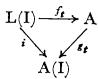
\includegraphics[keepaspectratio]{images/part001_16682a88.jpg}}

其中 \(i\) 是典范单射， \(f_{t}\) 是由 \(\pmb{t}\) 定义的李代数同态，而 \(g_{t}\) 是使得 \(g_{t}(i) = t_{i}\) （对 \(i\in I\) ）的幺代数同态。由于 \(g_{t}\circ i\) 与 \(f_{t}\) 在 I 上一致，该图表是交换的。由此得出，若 \(\mathrm{P}\in \mathrm{L}(\mathrm{I})\) ，则 § 2 no. 4 中定义的元素 \(\mathrm{P}((t_i)_{i\in I})\) 与《代数》第 III 章 § 2 no. 8 例 2 中定义的元素 \(\mathrm{P}((t_i)_{i\in I})\) 一致。

